%% Verze pro jednostranný tisk:
% Okraje: levý 40mm, pravý 25mm, horní a dolní 25mm
% (ale pozor, LaTeX si sám přidává 1in)
\documentclass[12pt,a4paper]{article}

% \openright zařídí, aby následující text začínal na pravé straně knihy
%\let\openright=\clearpage

%% Pokud tiskneme oboustranně:
% \documentclass[12pt,a4paper,twoside,openright]{report}
% \setlength\textwidth{145mm}
% \setlength\textheight{247mm}
% \setlength\oddsidemargin{14.2mm}
% \setlength\evensidemargin{0mm}
% \setlength\topmargin{0mm}
% \setlength\headsep{0mm}
% \setlength\headheight{0mm}
% \let\openright=\cleardoublepage

%% Vytváříme PDF/A-2u
\usepackage[a-2u]{pdfx}

%% Přepneme na českou sazbu a fonty Latin Modern
\usepackage[slovak]{babel}
\usepackage{lmodern}
\usepackage[IL2]{fontenc}%T1
\usepackage{textcomp}
\usepackage{hyperref}

\usepackage{float}
\usepackage{subfigure}

%% Použité kódování znaků: obvykle latin2, cp1250 nebo utf8:
\usepackage[utf8]{inputenc}

%%% Další užitečné balíčky (jsou součástí běžných distribucí LaTeXu)
\usepackage{amsmath}        % rozšíření pro sazbu matematiky
\usepackage{amsfonts}       % matematické fonty
\usepackage{amsthm}         % sazba vět, definic apod.

%bolo treba vypnut kvoli rozdelovaniu
%\usepackage{bbding}         % balíček s nejrůznějšími symboly
% (čtverečky, hvězdičky, tužtičky, nůžtičky, ...)
\usepackage{bm}             % tučné symboly (příkaz \bm)
\usepackage{graphicx}       % vkládání obrázků
\usepackage{fancyvrb}       % vylepšené prostředí pro strojové písmo
\usepackage{indentfirst}    % zavede odsazení 1. odstavce kapitoly
%\usepackage{natbib}         % zajištuje možnost odkazovat na literaturu
% stylem AUTOR (ROK), resp. AUTOR [ČÍSLO]
\usepackage[nottoc]{tocbibind} % zajistí přidání seznamu literatury,
% obrázků a tabulek do obsahu
\usepackage{icomma}         % inteligetní čárka v maltematickém módu
\usepackage{dcolumn}        % lepší zarovnání sloupců v tabulkách
\usepackage{booktabs}       % lepší vodorovné linky v tabulkách
\usepackage{paralist}       % lepší enumerate a itemize
\usepackage[usenames]{xcolor}  % barevná sazba

\usepackage{url}

\usepackage{pdfpages}
%opening
\title{}
\author{}

\begin{document}
	\pagestyle{empty}
\section{Transpozícia matice}

\subsection{Meranie času}

Ako prvé uvádzam meranie na mojom počítači: Intel Core i5-6600K@4.4GHz, 6MB cache, 16GB RAM, Windows 10.

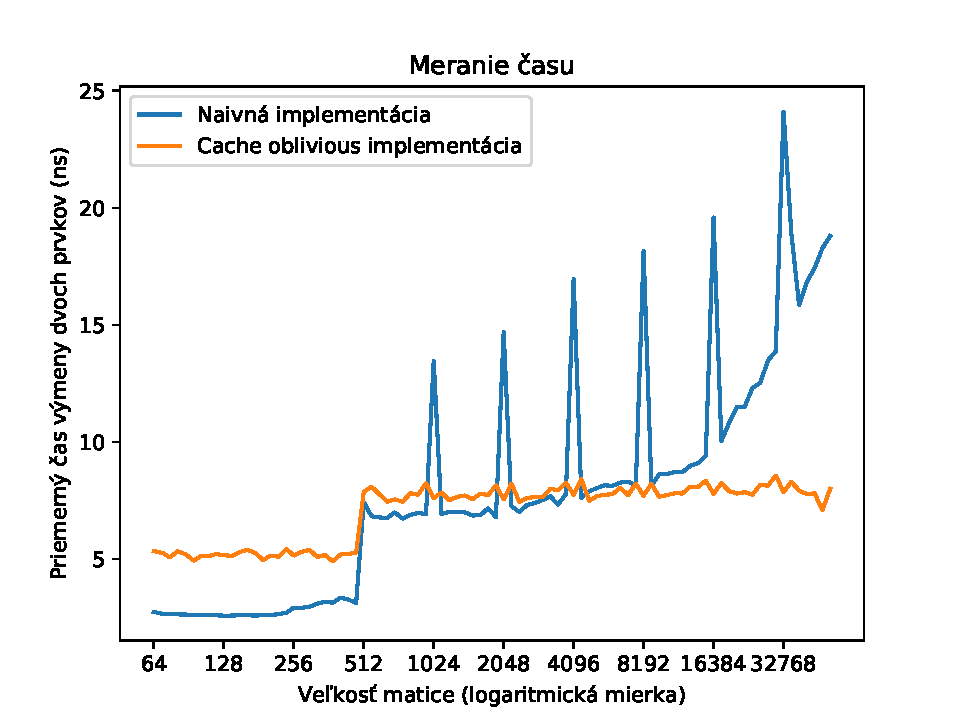
\includegraphics[width=\linewidth]{time-6600K.pdf}

\pagebreak

Ďalej uvádzam meranie na počítači v labe: Intel Core i7-6700@3.4 GHz, 8MB cache, 16GB RAM, linux.

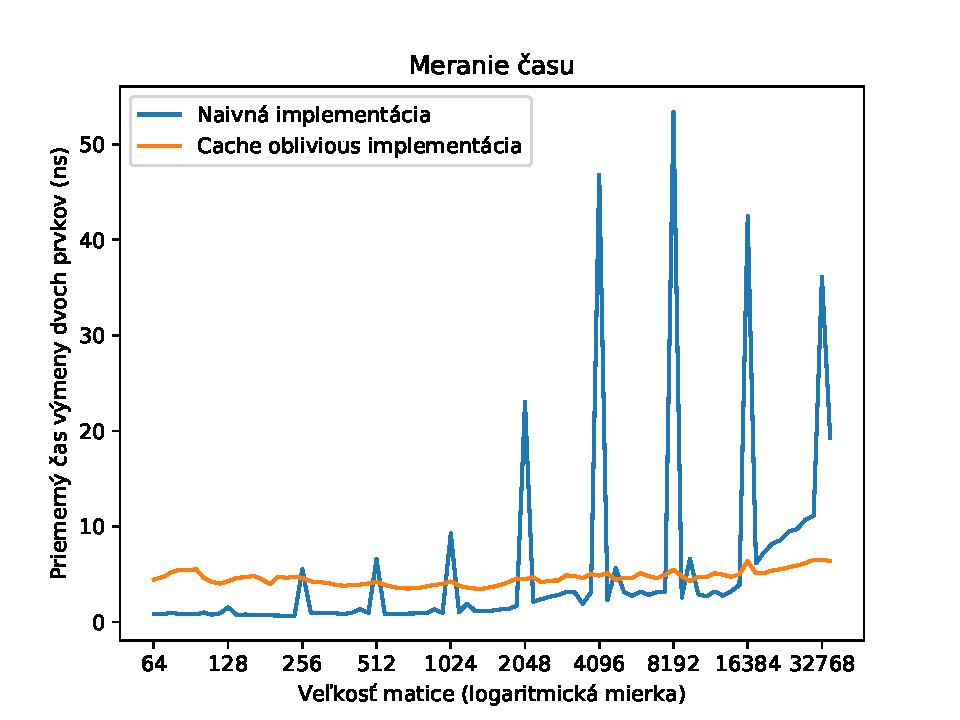
\includegraphics[width=\linewidth]{time-6700.pdf}

Môžeme pozorovať niekoľko vecí:
\begin{itemize}
	\item Na prvom grafe pozorujeme rovnako pri naivnom aj rekurzívnom algoritme veľký skok pri veľkosti matice 512. Vtedy má matica 512*512*4=1MB, čo nie je veľkosť žiadnej z keší (L1 má 32~kB, L2~256 kB, L3~6~MB). Je tiež zvláštne, že skok nastane pri \emph{oboch} algoritmoch. Bohužiaľ sa mi nepodarilo nájsť odpoveď na to, prečo to tak je. Na počítači v labe som nič také nenameral, a tak si myslím, že je to niečo špecifické pre implementáciu procesoru, prekladača, alebo operačného systému, a ďalej sa tým v analýze nebudem zaoberať.
	\item Priemerný čas jednej výmeny rekurzívneho cache-oblivious algoritmu (podľa očakávania) nezáleží na veľkosti matice.
	\item Naivný algoritmus sa správa zle, ak je počet riadkov N matice mocninou 2. To sa deje kvôli tomu, že cache procesoru nie je plne asociatívna. Pri iterovaní vnútorného cyklu postupne pristupujeme ku prvej, druhej, až poslednej N-tej bunke toho istého stĺpca matice. Keďže je matica uložená po riadkoch, tak to znamená, že pri posune o jeden riadok dolu skočíme v pamäti o N buniek pamäte. Ak je však N násobkom počtu blokov cache, tak kvôli obmedzenej asociativite cache sa začnú vyhadzovať z cache bloky z toho istého stĺpca, hoci je zaplnený iba zlomok celkovej veľkosti cache.
	\item Na oboch grafoch vidíme, že naivný algoritmus je rýchly, pokiaľ sa dostatočne veľká časť matice zmestí do cache. Do cache sa nemusí zmestiť celá matica, algoritmus však potrebuje, aby sa do cache zmestil stĺpec blokov cache, a korešpondujúce riadky (potrebujeme toľko riadkov, koľko je dĺžka jedného riadku/bloku cache). Vtedy je počet cache miss minimálny. Na grafoch vidíme, že pre väčšie N už počet cache miss narastá a tým aj čas na jednu výmenu.
\end{itemize}

\section{Simulátor}

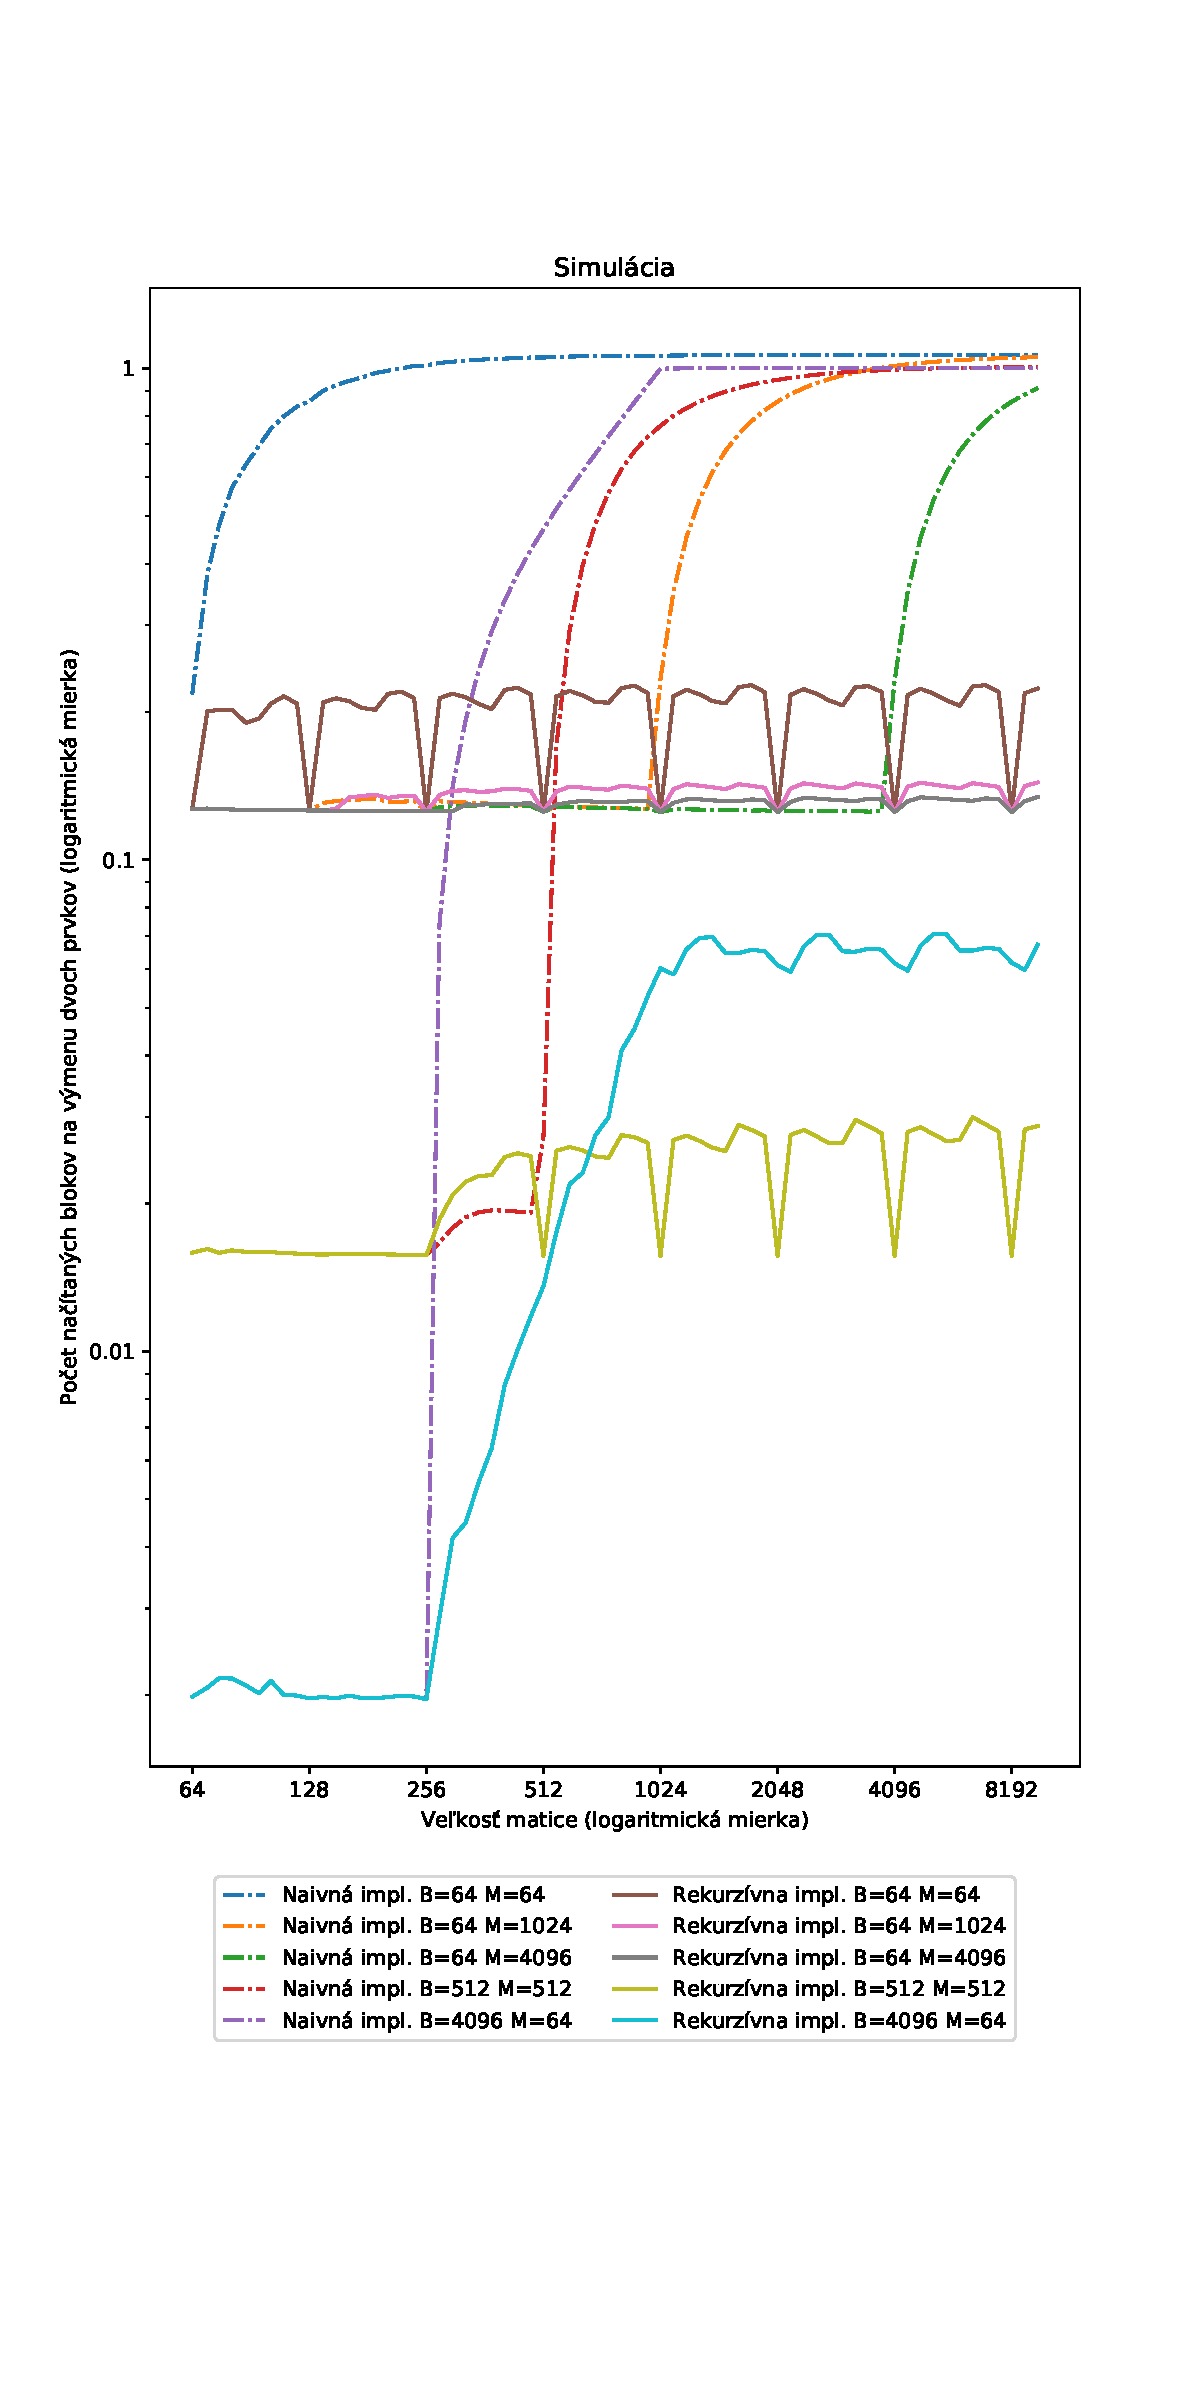
\includegraphics[width=\linewidth]{sim.pdf}

\begin{itemize}
	\item Vidíme, že kým je matica menšia ako veľkosť cache, nie sú medzi algoritmami žiadne rozdiely: pre (B=64,M=64) túto situáciu graf nezachytáva, pre (B=64,M=1024) je to pre N=128, teda matica má 128*128*4 B = 64*1024 B. Pre zvyšné verzie parametre cache to nastáva pri N=256, keď cache má 256~kB
	\item Po tomto bode už záleží na parametroch cache. Napráklad aj naivný algoritmus pre cache (B=64,M=4096) a (B=64,M=1024) sa správa dobre, pretože sa tu uplatní vyššie popísaný princíp toho, že naivný algoritmus potrebuje, aby sa do cache zmestilo iba niekoľko stĺpcov a prislúchajúcich riadkov v závislosti od dĺžky bloku. Naproti tomu cache (B=4096,M=64) a čiastočne (B=512,M=512) nemajú dosť blokov aby poskytli naivnému algoritmu dobré správanie už pre malé veľkosti matice.
	\item Vidíme potvrdenie analýzy z prednášky, že naivný algoritmus potrebuje až $N^2$ prístupov do cache: Pre akékoľvek parametre cache sa krivky naivných algoritmov blížia k 1 s rastúcim N.
	\item Cache-oblivious algoritmus má menej cache missov, keď je N mocninou 2. To je pravdepodobne spôsobené tým, že podštvorce matice, ktoré sú spracovávané rekurzívne a bloky cache sú zarovnané, a teda sa nestáva, že blok, z ktorého sme potrebovali iba časť v predchodzom štvorci, načítame ešte raz v nasledujúcom (samozrejme pre štvorce väčšie ako jeden blok cache).
\end{itemize}

\end{document}